\begin{figure}[H]
	\centering
	\scalebox{0.7}{% XCircuit output "config6.tex" for LaTeX input from config6.ps
\def\putbox#1#2#3#4{\makebox[0in][l]{\makebox[#1][l]{}\raisebox{\baselineskip}[0in][0in]{\raisebox{#2}[0in][0in]{\scalebox{#3}{#4}}}}}
\def\rightbox#1{\makebox[0in][r]{#1}}
\def\centbox#1{\makebox[0in]{#1}}
\def\topbox#1{\raisebox{-0.60\baselineskip}[0in][0in]{#1}}
\def\midbox#1{\raisebox{-0.20\baselineskip}[0in][0in]{#1}}
   \scalebox{1}{
   \normalsize
   \parbox{6.91667in}{
   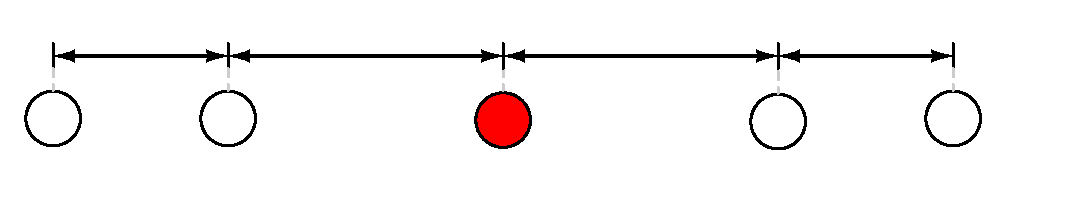
\includegraphics[scale=1]{config6}\\
   % translate x=548 y=272 scale 0.38
   \putbox{3.2in}{0.08in}{1.20}{$\lambda$}%
   \putbox{4.99in}{0.06in}{1.20}{$\lambda/2$}%
   \putbox{2.04in}{0.97in}{1.20}{$\lambda/2$}%
   \putbox{1.22in}{0.08in}{1.20}{$\lambda/2$}%
   \putbox{6.1in}{0.08in}{1.20}{$\lambda/4$}%
   \putbox{0.66in}{0.97in}{1.20}{$\lambda/4$}%
   \putbox{5.5in}{0.95in}{1.20}{$\lambda/4$}%
   \putbox{0.06in}{0.08in}{1.20}{$\lambda/4$}%
   \putbox{4in}{0.95in}{1.20}{$\lambda/2$}%
   } % close 'parbox'
   } % close 'scalebox'
   \vspace{-\baselineskip} % this is not necessary, but looks better
}
	\caption{Configuración 6 asignada en dirección $z$.}
	\label{fig.config_z}
\end{figure}	


La figura \ref{fig.config_z} muestra la configuración de radiadores asignada vista desde arriba (plano xy), la misma consiste en un conjunto de conductores formada por alambres, de los cuales sólo uno de ellos (de color rojo) es activo, es decir se encuentra conectado a una funete de tensión de \SI{1}{\volt}. Los cuatro conductores restantes son pasivos, pudiendo funcionar como directores o reflectores. El radio de todos los conductores es de \SI{5}{\milli\meter}.
La longitud y distancias entre conductores están expresadas en términos de longitud de onda para la frecuencia más pequeña. El rango de fercuencias a analizar es $\SI{80}{\mega\hertz} < f < \SI{480}{\mega\hertz}$, por lo que se puede deducir el valor de una longitud de onda según la expresión \eqref{ec.long_onda}, sinedo $\rm{c}=\SI{3e8}{\meter\per\second}$ la velocidad de propagación de la onda en espacio libre.

\begin{equation}
	\centering
	\lambda = \frac{\rm{c}}{\rm{f_{min}}} = \frac{ \SI{3e8}{\meter\per\second} } { \SI{80}{\mega\hertz} } = \SI{3.75}{\meter}
	\label{ec.long_onda}
\end{equation} 

\begin{figure}[H]
	\begin{subfigure}{0.5\textwidth}
		\scalebox{0.7}{% XCircuit output "config6xy.tex" for LaTeX input from config6xy.ps
\def\putbox#1#2#3#4{\makebox[0in][l]{\makebox[#1][l]{}\raisebox{\baselineskip}[0in][0in]{\raisebox{#2}[0in][0in]{\scalebox{#3}{#4}}}}}
\def\rightbox#1{\makebox[0in][r]{#1}}
\def\centbox#1{\makebox[0in]{#1}}
\def\topbox#1{\raisebox{-0.60\baselineskip}[0in][0in]{#1}}
\def\midbox#1{\raisebox{-0.20\baselineskip}[0in][0in]{#1}}
   \scalebox{1}{
   \normalsize
   \parbox{4.1875in}{
   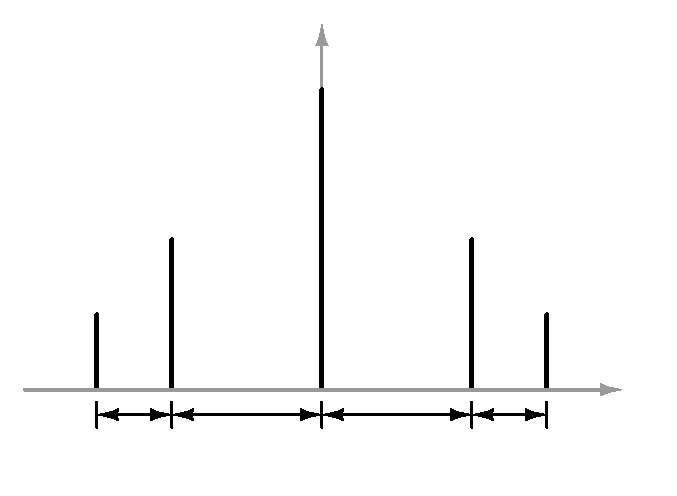
\includegraphics[scale=1]{config6xy}\\
   % translate x=540 y=424 scale 0.38
   \putbox{1.85in}{0.7in}{1.20}{\rotatebox{-270}{\tiny{$\lambda = \SI{3.75}{\meter}$}}}%
   \putbox{0.85in}{0.7in}{1.20}{\rotatebox{-270}{\tiny{$\lambda /2 = \SI{1.875}{\meter}$}}}%
   \putbox{0.35in}{0.7in}{1.20}{\rotatebox{-270}{\tiny{$\lambda /4 = \SI{0.9375}{\meter}$}}}%
   \putbox{2.85in}{0.7in}{1.20}{\rotatebox{-270}{\tiny{$\lambda /2 = \SI{1.875}{\meter}$}}}%
   \putbox{3.4in}{0.7in}{1.20}{\rotatebox{-270}{\tiny{$\lambda /4 = \SI{0.9375}{\meter}$}}}%
   \putbox{2.14in}{2.89in}{1.20}{$z$}%
   \putbox{4.14in}{0.56in}{1.20}{$x$}%
   \putbox{1.2in}{0.26in}{1.20}{{\tiny{$\lambda /2 = \SI{1.875}{\meter}$}}}%
   \putbox{2.2in}{0.26in}{1.20}{{\tiny{$\lambda /2 = \SI{1.875}{\meter}$}}}%
   \putbox{0.58in}{0.26in}{1.20}{\tiny{$\lambda /4=$}}%
   \putbox{3.18in}{0.26in}{1.20}{\tiny{$\lambda /4=$}}%
   \putbox{0.5in}{0.15in}{1.20}{\tiny{$\SI{0.9375}{\meter}$}}%
   \putbox{3.1in}{0.15in}{1.20}{\tiny{$\SI{0.9375}{\meter}$}}%
   } % close 'parbox'
   } % close 'scalebox'
   \vspace{-\baselineskip} % this is not necessary, but looks better
}
		\caption{Configuración 6 asignada (plano $xz$).}
		\label{fig.config_xz}
	\end{subfigure}
	\quad
	\begin{subfigure}{0.5\textwidth}
		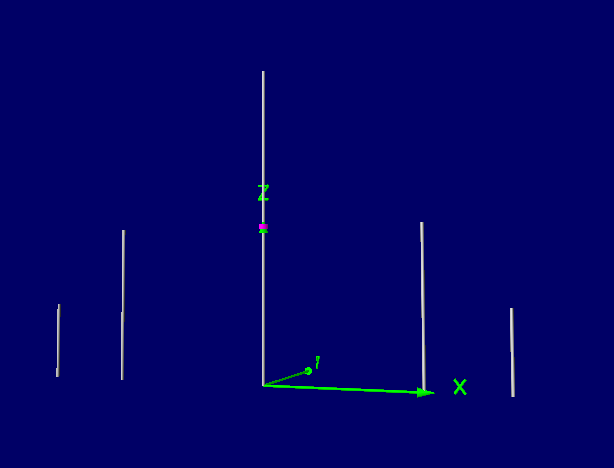
\includegraphics[scale=0.4]{imagenes/2_geometria.png}
		\caption{Geometría ingresada en el programa \textit{4nec2}.}
		\label{fig.geometria}
	\end{subfigure}
\end{figure}
 
Por lo tanto la configuración en el plano xz con las medidas correspondientes se muestra en \ref{fig.config_xz}. La figura \ref{fig.geometria} muestra la geometría ingresada en el programa \textit{4nec2}, en espacio libre. El punto rosa en el conductor central indica la fuente (que es de \SI{1}{\volt}) y se ubicó en su posición central.   







